%!TEX root = main.tex



%We are ready to define prioritized streaming string transducers. 
%In the definition, 
%
%The special symbol $\nullchar$ is introduced to capture the situation that $\extract_{i,e}(x)$ returns $\nullchar$, i.e. $x \in \Lang(e)$ but the $i$-th capturing group of $e$ is not matched.
%

\paragraph{Semantics}
We now define the formal semantics of $\regexp$. Traditionally, regular expressions are interpreted as a regular language, i.e., a set of strings, which can be defined inductively in a rather straightforward way. In our case when the regular expression is used in string constraints arisen from analysis of programming language such as JavaScript, %owing to the introduction of greedy/lazy semantics,  
what we need is not only the language denoted by the regular expression, but also the intermediate result when parsing a string against the given regular expression. This is especially the case when the capturing group is involved. As a result, we need a more operational (as opposed traditional denotational) account of the semantics for regular expression. To this end, we harness an extension of finite-state automata with priorities, which \emph{defines} how a string is accepted by the given regular expression. We start with the standard finite-state automaton.  


%\subsection{Semantics of \regexp[\sf CG]}
%In this section, we give one of the many semantics of \regexp[\sf CG], which we will utilize for $\replaceall$.
%For two indexed $\regexp$s $e$ and $e'$, we say $e'$ is a \emph{subexpression} of $e$,
%if one of the following conditions holds: 1) $e'=e$, 2) $e = [e_1 \cdot e_2]$ or $[e_1 + e_2]$, and $e'$ is a subexpression of $e_1$ or $e_2$, 3) $e = [e^?], [e^{??}], [e_1^{\ast}]$, $[e_1^{+}]$, $[e_1^{\ast?}]$, $[e_1^{+?}]$, $e_1^{\{m_1, m_2\}}$, $e_1^{\{m_1, m_2\}?}$ or $(_n e_1)_n$, and $e'$ is a subexpression of $e_1$. We use $S(e)$ to denote the set of all subexpressions of $e$. %\tl{is there a difference between $[e_1\cdot e_2]$ and $e_1 e_2$?}
%
% 
%By a mutual induction on $|w|$ and $|e|$, we can show that $|\cM_{w}(e)|$, the size of $\cM_{w}(e)$, is at most $|w||e|$.  

%\begin{example}\label{exmp-regex-match-tree}
%	Let $w= 0250$ and $e = [[([\Gamma^+])\concat .?] \concat ([\Gamma^*])]$ where $\Gamma = \{0,1,\cdots,9\}$. Note that $e$ is essentially {\tt decimalReg} in the motivating example. Then $\cM_{w}(e) = \{T_1,T_2,T_3, T_4\}$ as illustrated in Figure~\ref{fig-regex-semantics-decimal}(i), (ii), (iii), and (iv), where the match trees rooted at $(0, \Gamma)$, $(2, \Gamma)$, and $(5, \Gamma)$ are omitted. % to avoid tediousness.
%	\begin{figure}[htb]
%		\centering
%		%\rule{\linewidth}{0cm}
%		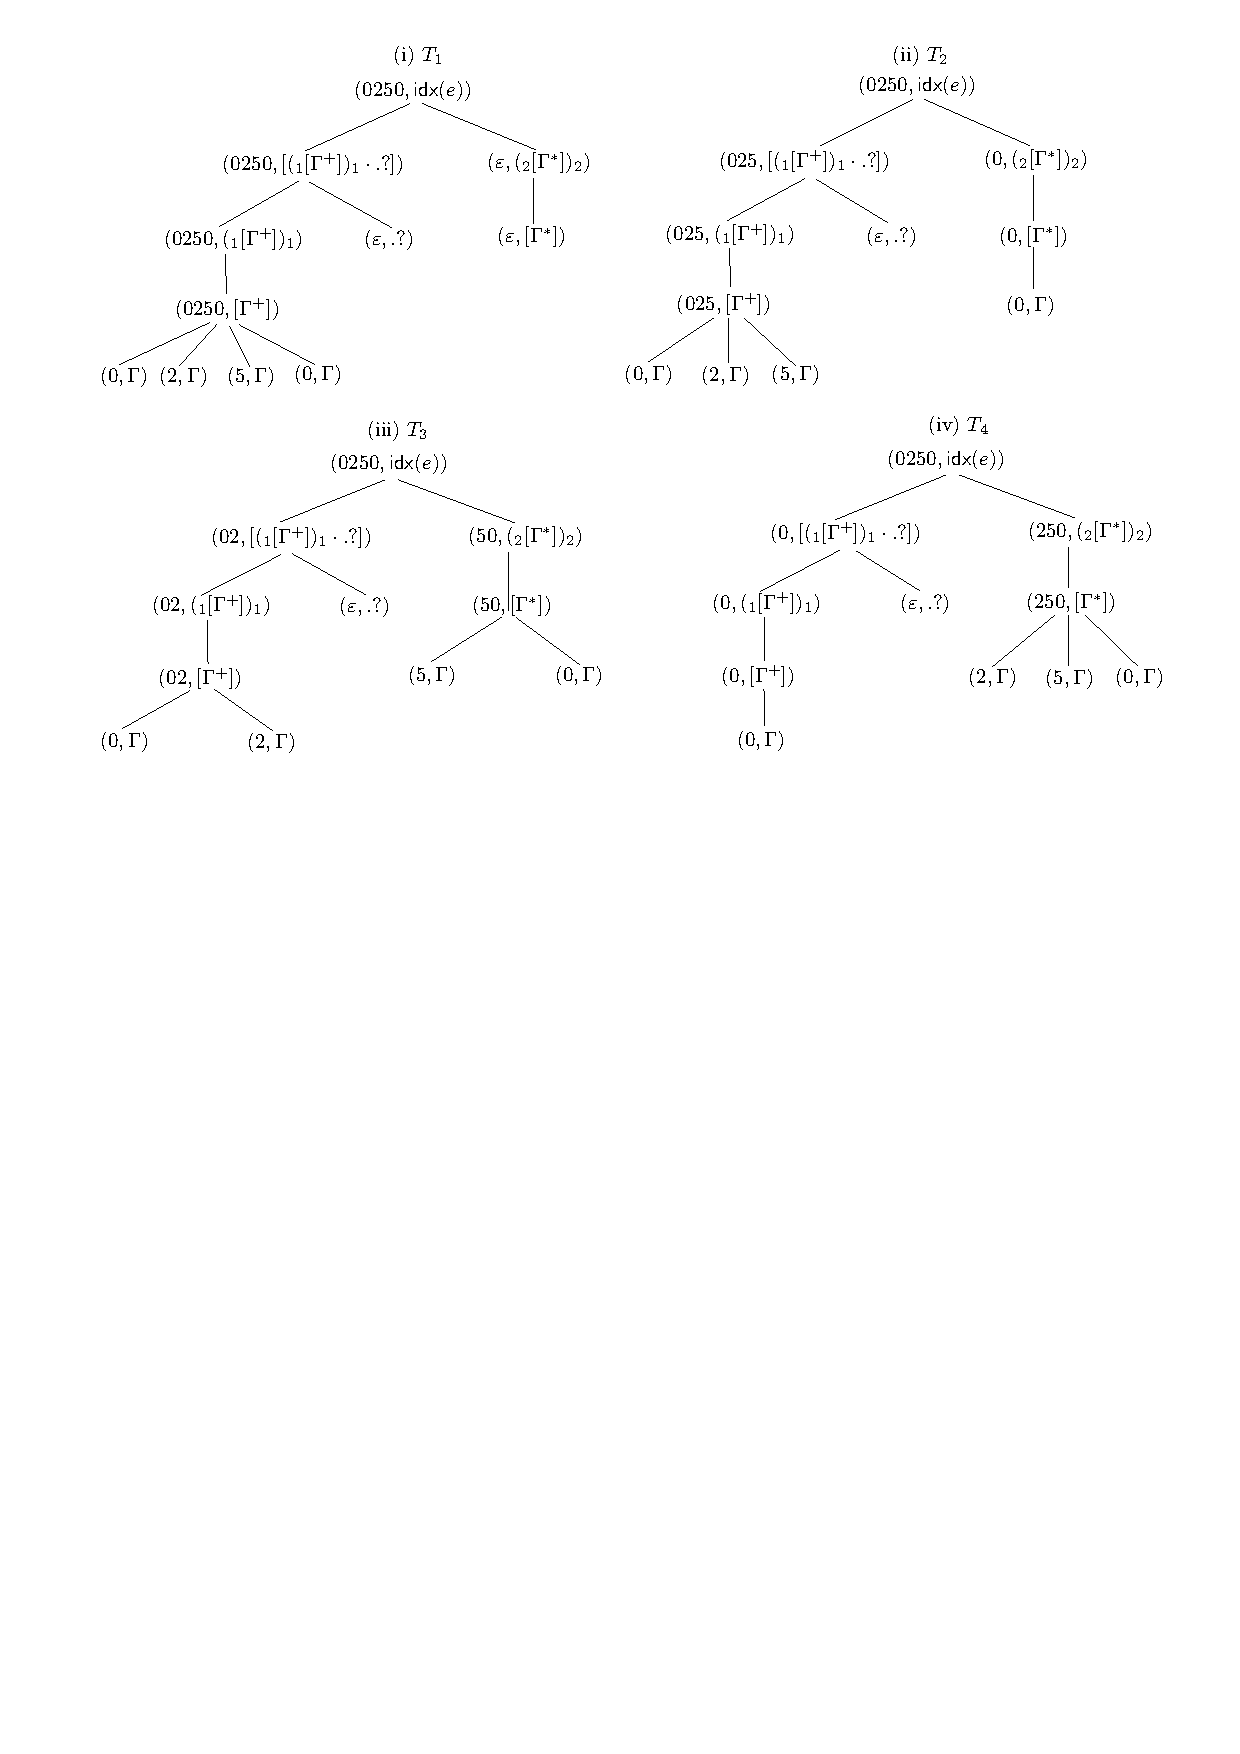
\includegraphics[width=1\textwidth]{regex-semantics-decimal.pdf}
%		\caption{Match trees of $e=[[([\Gamma^+])\concat .?] \concat ([\Gamma^*])]$ to $w= 0250$}
%		\label{fig-regex-semantics-decimal}
%		
%	\end{figure}
%	%\Blindtext
%\end{example}

 
 
%
%\begin{example}\label{exmp-regex-semantics}
%	Let us continue Example~\ref{exmp-regex-match-tree}.  In Fig.~\ref{fig-regex-semantics-decimal}, we have $(T_1)_{(0250, [\Gamma^+])} >_{(w, \idxexp(e))} (T_2)_{(025, [\Gamma^+])}$, since $(0, \Gamma)(2, \Gamma)(5,\Gamma)$ is a proper prefix of $(0, \Gamma)(2, \Gamma)(5,\Gamma)(0, \Gamma)$. Then we deduce that $(T_1)_{(0250, (_1[\Gamma^+])_1)} >_{(w, \idxexp(e))} (T_2)_{(025, (_1[\Gamma^+])_1)}$. Consequently, $(T_1)_{(0250, [(_1[\Gamma^+])_1 \concat .?])} >_{(w, \idxexp(e))} (T_2)_{(025,  [(_1[\Gamma^+])_1 \concat .?])}$ and $T_1 >_{(w, \idxexp(e))} T_2$. Similarly, we have $T_2 >_{(w, \idxexp(e))} T_3$ and $T_3 >_{(w, \idxexp(e))} T_4$. Therefore, $T_1$ is the accepting match of $e$ to $w$, where the first and second capturing group of $e$ are matched to $0250$  and $\varepsilon$ respectively. 
%	%\Blindtext
%\end{example}

%\begin{remark}
%	Our semantics of $\regexp$ follows the 11th Edition of the ECMAScript specification (ES11 for short) \cite{ECMAScript11}, with a focus on the non-commutative union, the greedy/lazy semantics of Kleene star/plus, as well as capturing groups and backreferences.
%	In comparison, POSIX regular expressions require the leftmost and longest match of regular expressions, which we leave as future work.
%\end{remark}


% some examples

%  e = b(a*)a*
%  
%  e' = b(a*?)a*

%\begin{figure}[ht]
%\centering
%\rule{\linewidth}{0cm}
%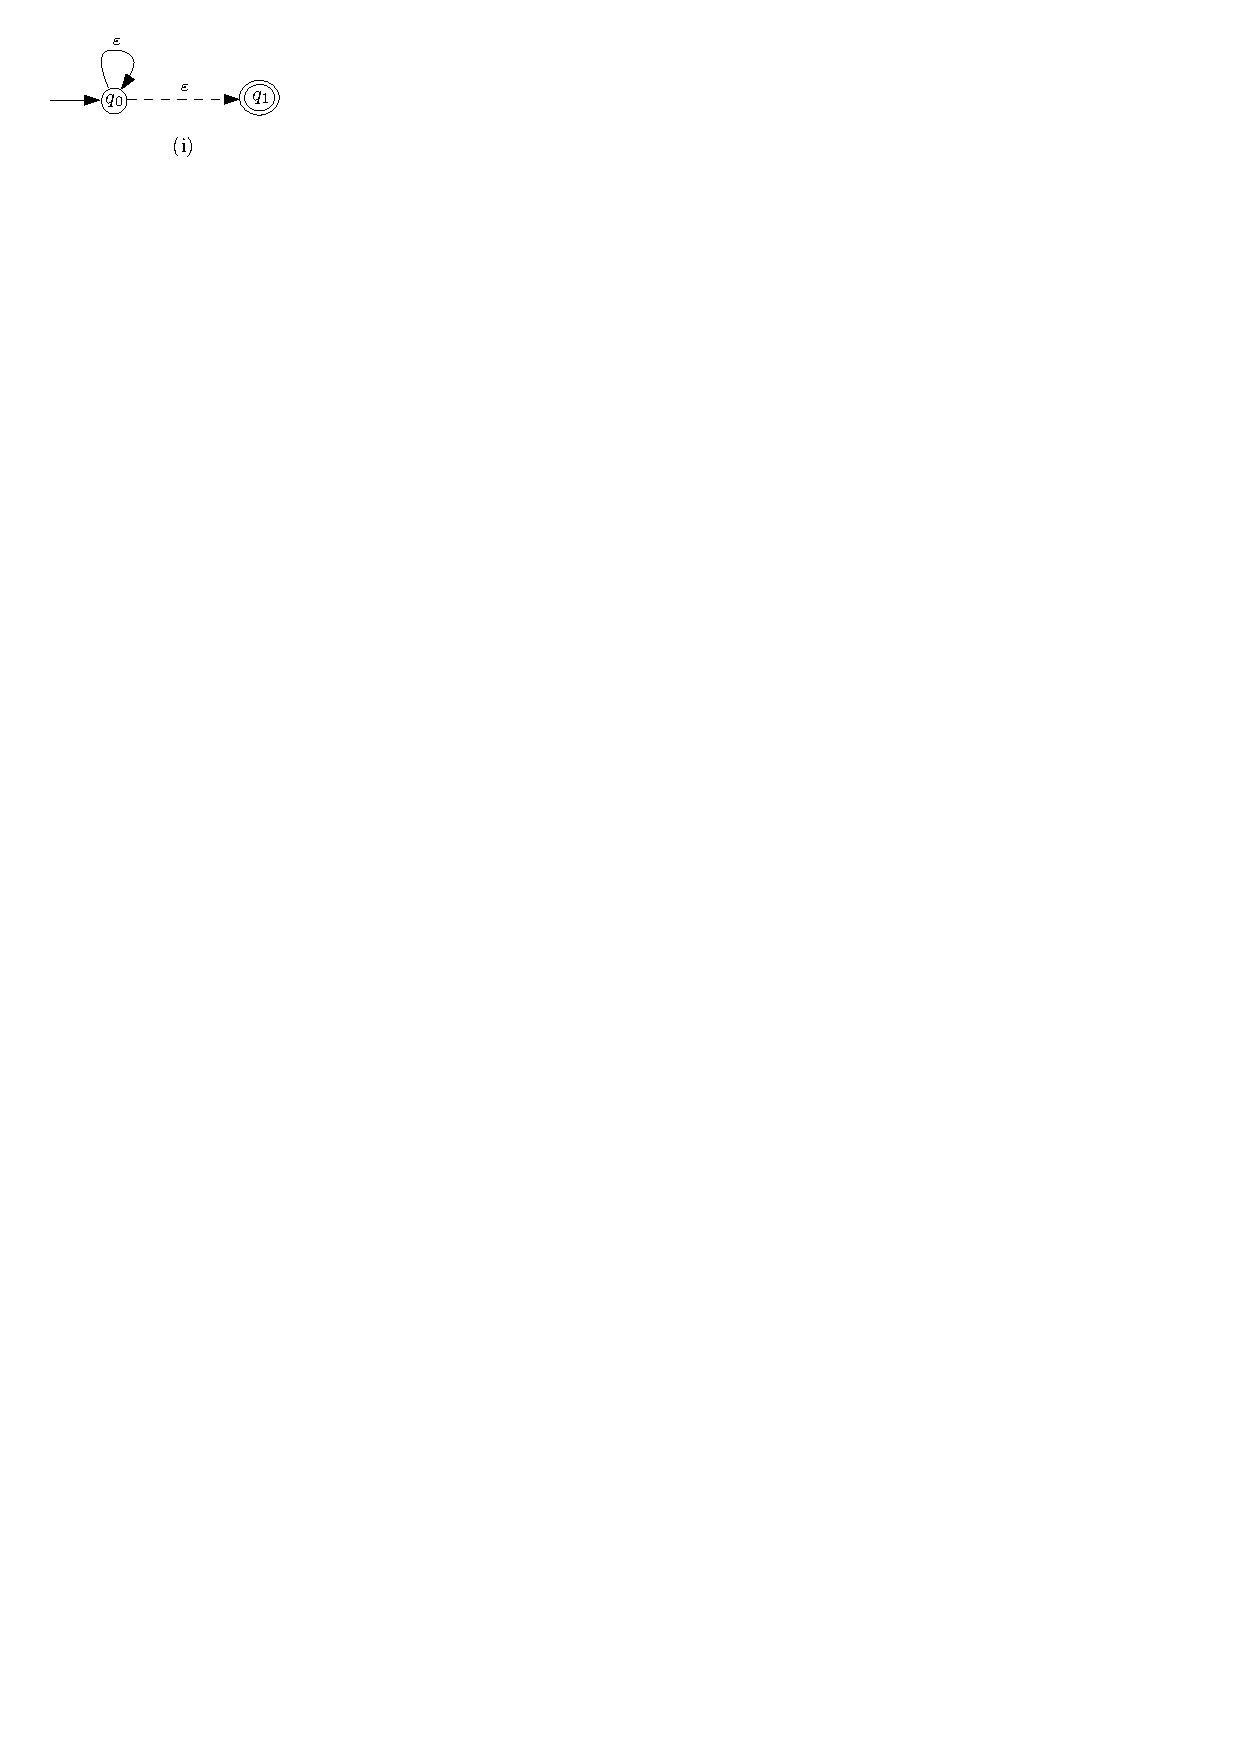
\includegraphics[scale=0.8]{pfa-epsilon-star.pdf}
%\caption{The PFA for $\varepsilon^\ast$}
%\label{fig-pfa-epsilon-star}
%\end{figure}



%%%%%%%%%%%%%%%%%%%%%%%%%%%%%%%%%%%%%%%%%%%%%%%%%%%%%%%%%%%%%%%%%%%%%%%%%%%%%%%%%%%%%%%%%%%%

%We can adapt the PFA construction in \cite{BDM14}, which in turn is a variant of the standard Thompson construction \cite{Thompson68}, and show the following result. 

%\begin{proposition}\label{prop-rwre-to-pfa}

%We associate with each regular expression $e$ a PFA $\cA_e$ and define the semantics of $e$ as the language accepted by $\cA_e$. As expected, the PFA $\cA_e$ is constructed inductively. 

\paragraph{Case $e =\emptyset$} $\cA_e = (\{q_{\emptyset, 0}\}, \Sigma, \emptyset, \delta, \tau, \emptyset, q_{\emptyset, 0}, (\emptyset, \emptyset))$, where $\delta(q_{\emptyset, 0}, a) = ()$ for every $a \in \Sigma$; $\tau(q_{\emptyset, 0}) = ((); ())$.
		

\paragraph{Case $e = \varepsilon$} $\cA_e = (\{q_{\varepsilon, 0}, f_{\varepsilon,0}\}, \Sigma, \{x \}, \delta, \tau, E, q_{\varepsilon,0}, (\{f_{\varepsilon,0}\}, \emptyset))$, 
%
where $\delta(q_{\varepsilon,0}, a) = \delta(f_{\varepsilon,0}, a) = ()$ for every $a \in \Sigma$; $\tau(q_{\varepsilon,0}) = ((f_{\varepsilon,0}); ())$;  $\tau(f_{\varepsilon,0}) = ((); ())$; for each transition $(q, a, q')$, $E(q,a,q')(x) =xa$.
		
\paragraph{Case $e = a$} $\cA_e = (\{q_{a,0}, q_{a,1}, f_{a,0}\}, \Sigma, \{x\}, \delta, \tau, E, q_{a,0}, (\emptyset, \{f_{a,0}\}))$, where 
$\delta(q_{a,0}, b) = ()$ for every $b \in \Sigma$, $\delta(q_{a,1}, a) = (f_{a,0})$, $\delta(q_{a,1}, b) = ()$ for every $b \in \Sigma \setminus \{a\}$; 
%
$\tau(q_{a,0}) = ((q_{a,1}); ())$, $\tau(q_{a,1}) = ((); ())$, and $\tau(f_{a,0}) = ((); ())$; 
%
for each transition $(q, a, q')$, $E(q,a,q')(x) =xa$.
%		
\begin{figure}[ht]
			\centering
			%\rule{\linewidth}{0cm}
			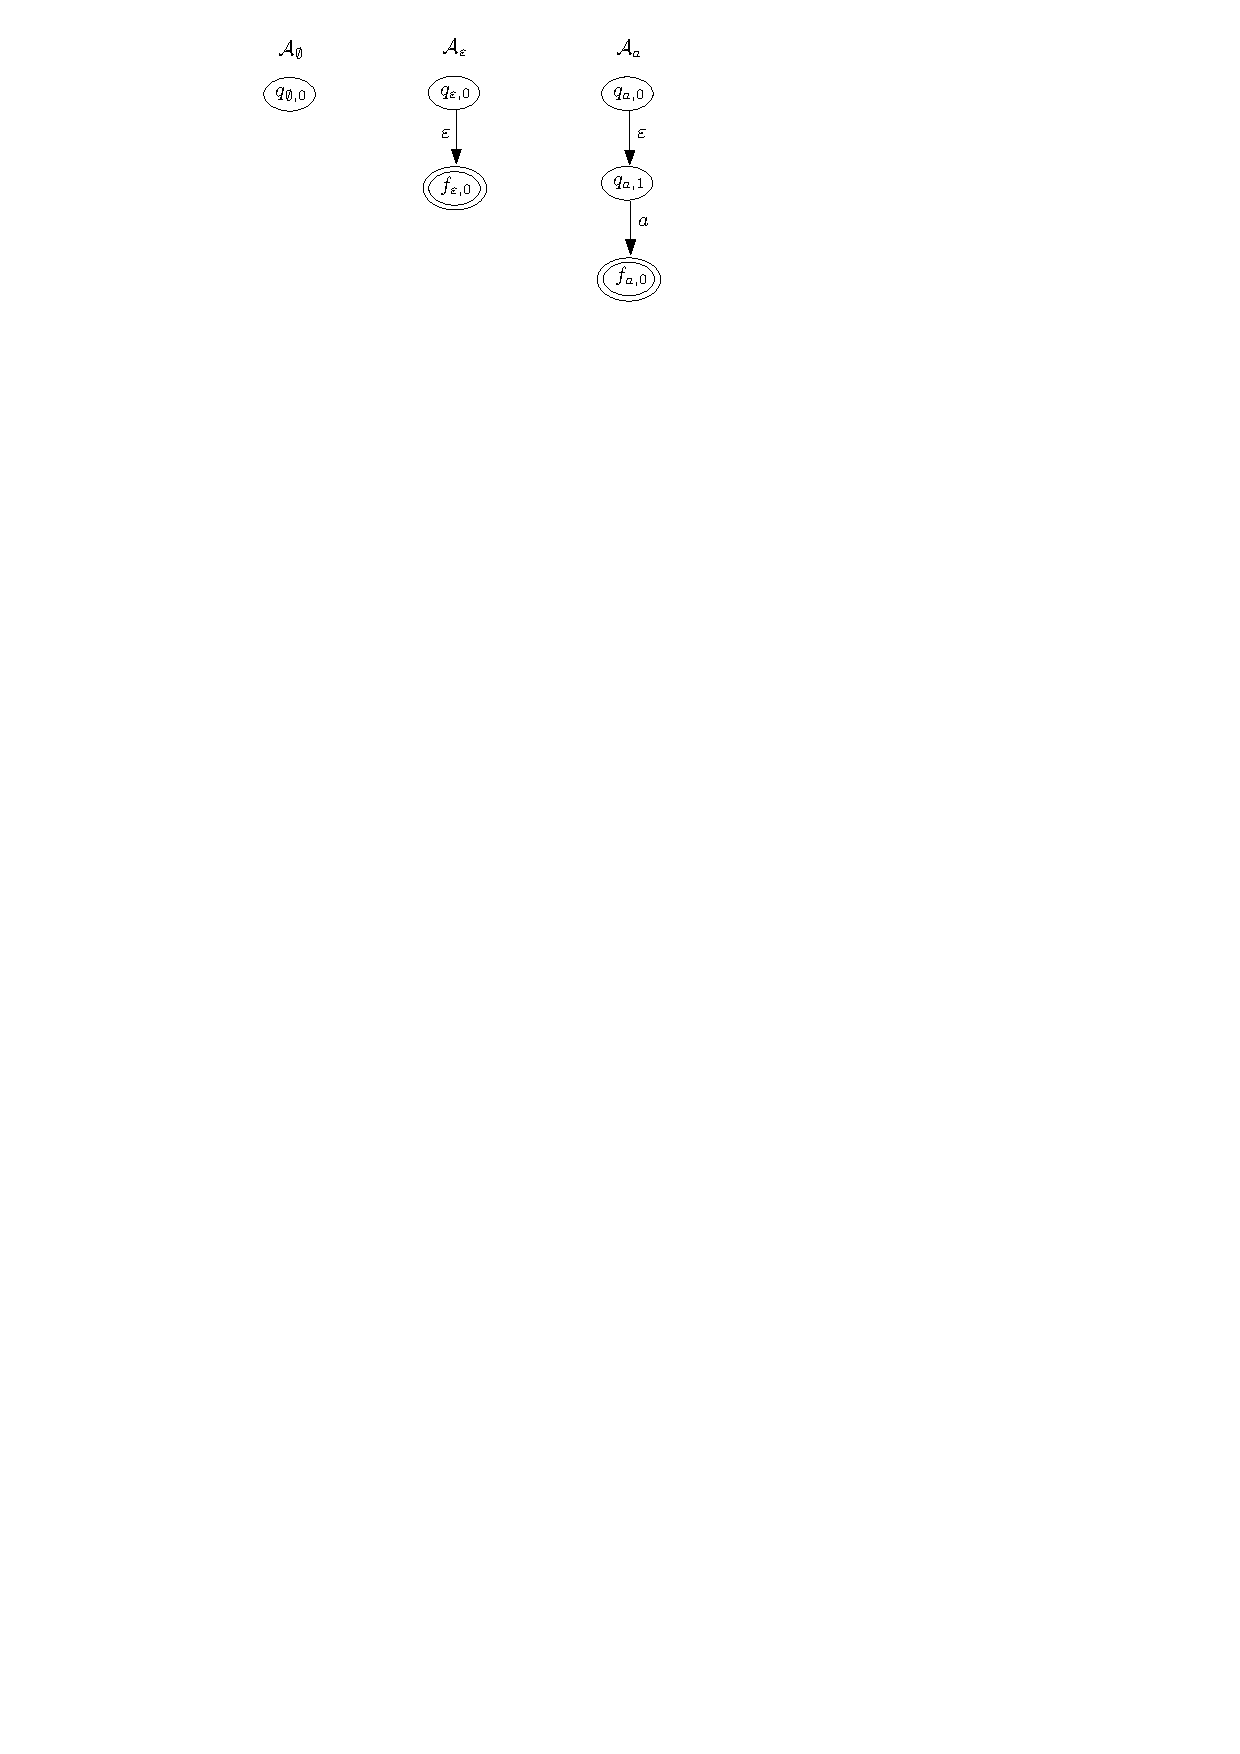
\includegraphics[width = 0.4\textwidth]{reg2pfa-0.pdf}
			\caption{The PFA $\cA_{\emptyset}$, $\cA_{\varepsilon}$, and $\cA_{a}$ }
			\label{fig-reg2pfa-0}
\end{figure}  
%%%%%%%%%%%%%%%%%%%%%%%%%%%%%%%%%%%%%%%%%%%%%%%%%%%%%%%%%%%%%%%%%%%%%%%%%%%%%%%%%%%%%%%%%%%%%%%%%%%%

		
\paragraph{Case $e = (e_1)$} $\cA_e = \cA_{e_1}$.
		

\paragraph{Case $e = [e_1 + e_2]$} Let 
\[\cA_{e_1} = (Q_{e_1}, \Sigma, X_1, \delta_{e_1}, \tau_{e_1}, E_1,  q_{e_1,0}, (F_{e_1,1}, F_{e_1,2}))\] and 
\[\cA_{e_2} = (Q_{e_2}, \Sigma, X_2, \delta_{e_2}, \tau_{e_2}, E_2, q_{e_2,0}, (F_{e_2, 1}, F_{e_2,2}))\] 
with $X_1\cap X_2=\emptyset$. 
Then 
\[\cA_e = (Q_{e_1} \cup Q_{e_2} \cup \{q_{e,0}\}, \Sigma, X_1\cup X_2, 
		\delta_e, \tau_e, E, q_{e,0}, (F_{e_1,1} \cup F_{e_2,1}, F_{e_1,2} \cup F_{e_2,2}))\] where  
		\begin{itemize}
			\item $q_{e,0}  \not \in Q_{e_1} \cup Q_{e_2}$, 
			\item $\delta_e(q, a) = \delta_{e_i}(q, a)$ for every $i \in \{1,2\}$, $q \in Q_{e_i}$ and $a \in \Sigma$, 
			$\delta_e(q_{e,0}, a)  = ()$ for every $a \in \Sigma$, 
			%
			\item $\tau_e(q) = \tau_{e_i}(q)$ for every $q \in Q_{e_i}$ ($i =1,2$), $\tau_e(q_{e,0}) = ((q_{e_1,0},q_{e_2,0}); ())$.
			\item for each transition $(q, a, q')$ from $\delta_i$ for $i\in\{1,2\}$, $E(q,a,q')(x) =xa$ and $E(q_{e,0},a,q')(x) =\varepsilon$
		\end{itemize}
Fig.~\ref{fig-reg2pfa-1} depicts the construction.  	
		\begin{figure}[ht]
			\centering
			%\rule{\linewidth}{0cm}
			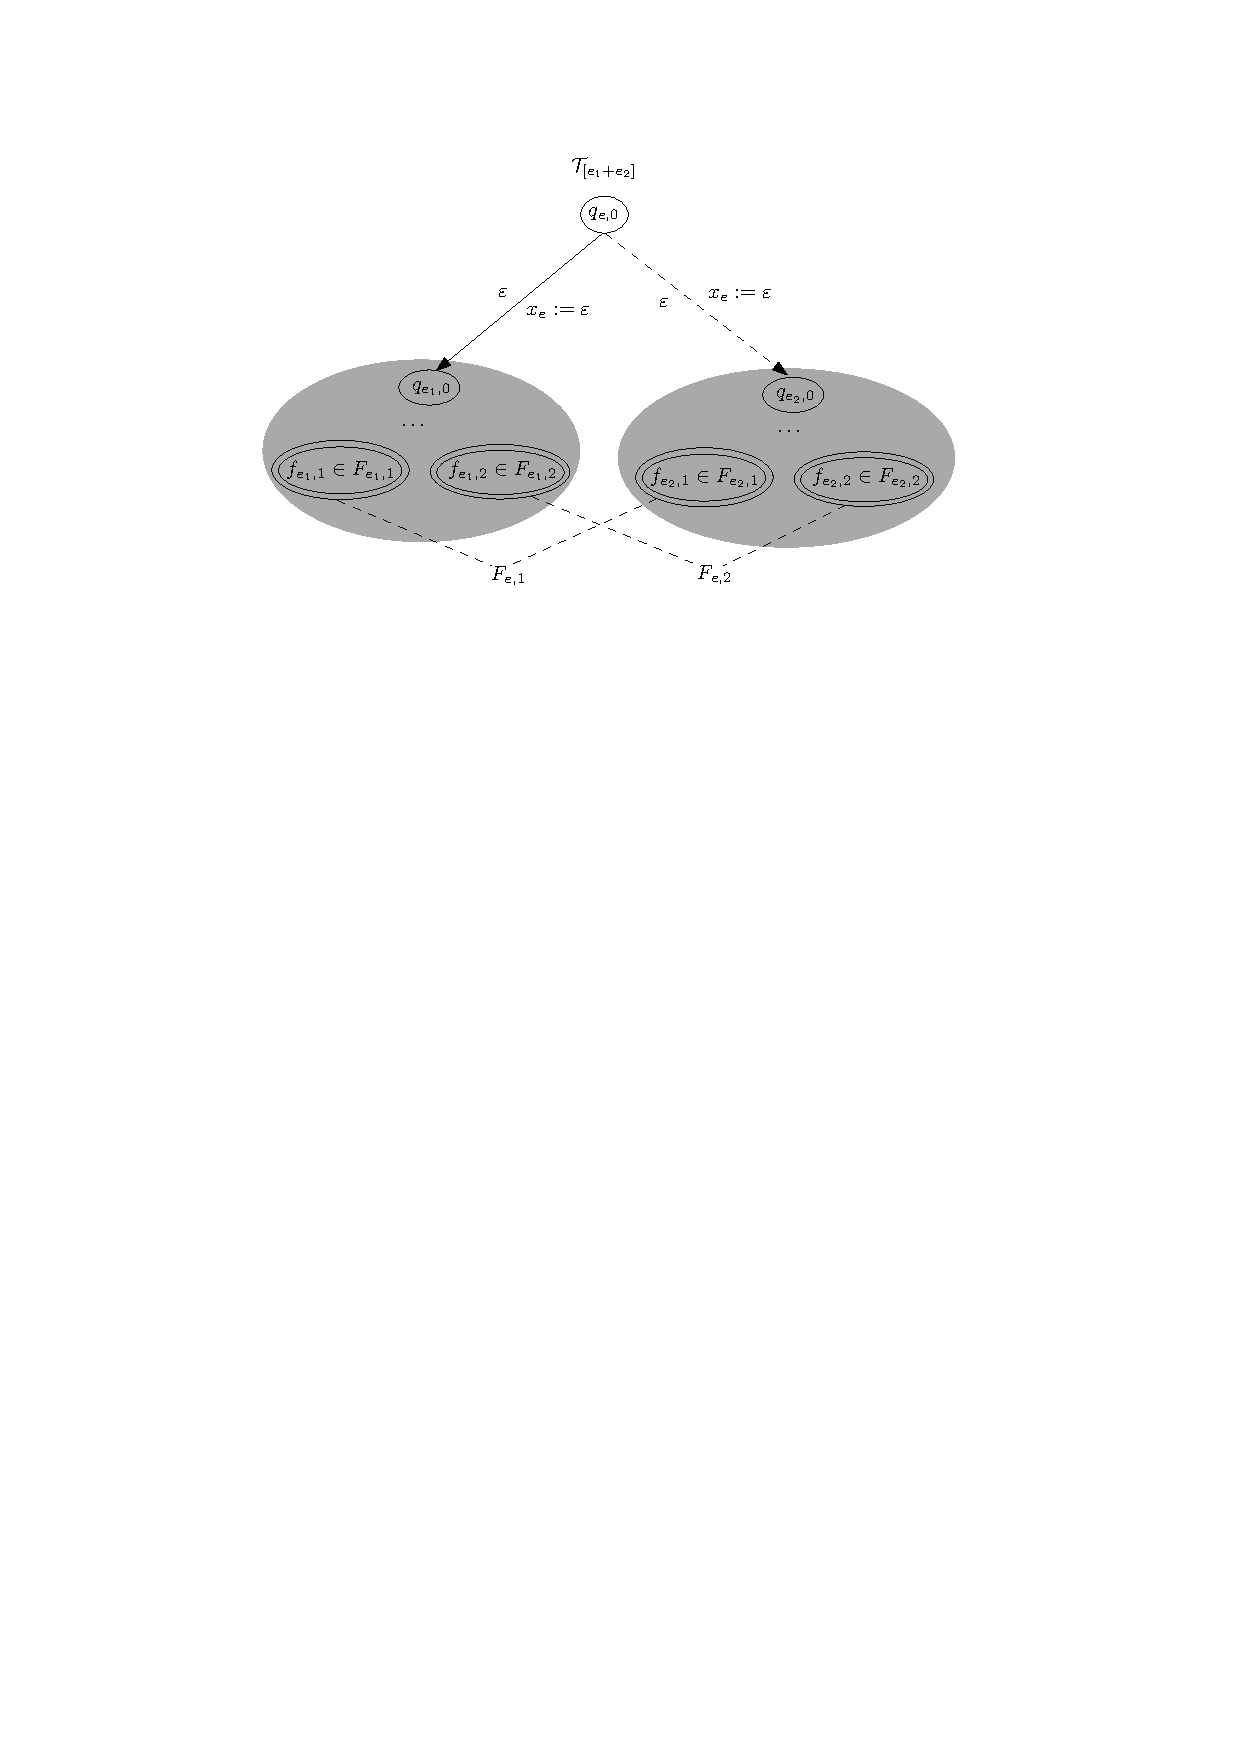
\includegraphics[width = 0.6\textwidth]{reg2pfa-1.pdf}
			\caption{The PFA $\cA_{[e_1+e_2]}$}
			\label{fig-reg2pfa-1}
		\end{figure}  

%%%%%%%%%%%%%%%%%%%%%%%%%%%%%%%%%%%%%%%%%%%%%%%%%%%%%%%%%%%%%%%%%%%%%%%%%%%%%%%%%%%%%%%%%%%%%%%%%%%%%

\paragraph{Case $e = [e_1^?]$} Let $\cA_{e_1} = (Q_{e_1}, \Sigma, X, \delta_{e_1}, \tau_{e_1}, E_1, q_{e_1,0}, (F_{e_1,1}, F_{e_1,2}))$. Then 
\[\cA_e = (Q_{e_1} \cup \{q_{\varepsilon}, q_{e,0}\}, \Sigma, X, 
		\delta_e, \tau_e, E, q_{e,0}, (\{q_{\varepsilon}\}, F_{e_1,2}))\]
where  
		\begin{itemize}
			\item $q_{e,0}  \not \in Q_{e_1}$
			\item $\delta_e(q, a) = \delta_{e_1}(q, a)$ for every $q \in Q_{e_1}$ and $a \in \Sigma$, $\delta_e(q_{e,0}, a)  = ()$ and $\delta_e(q_{\varepsilon}, a) = ()$ for every $a \in \Sigma$, 
			%
			\item $\tau_e(q) = \tau_{e_1}(q)$ for every $q \in Q_{e_1}$, $\tau_e(q_{e,0}) = ((q_{e_1,0},q_{\varepsilon}); ())$,
			\item for each transition $(q, a, q')$ from $\delta_{e_1}$, $E(q,a,q')(x) =E_1(q, a,q')$ and $E(q_{e,0},\varepsilon,q_{\varepsilon})(x) =\varepsilon$
		\end{itemize}
%
Fig.~\ref{fig-reg2pfa-6} depicts the construction.
		\begin{figure}[ht]
			\centering
			%\rule{\linewidth}{0cm}
			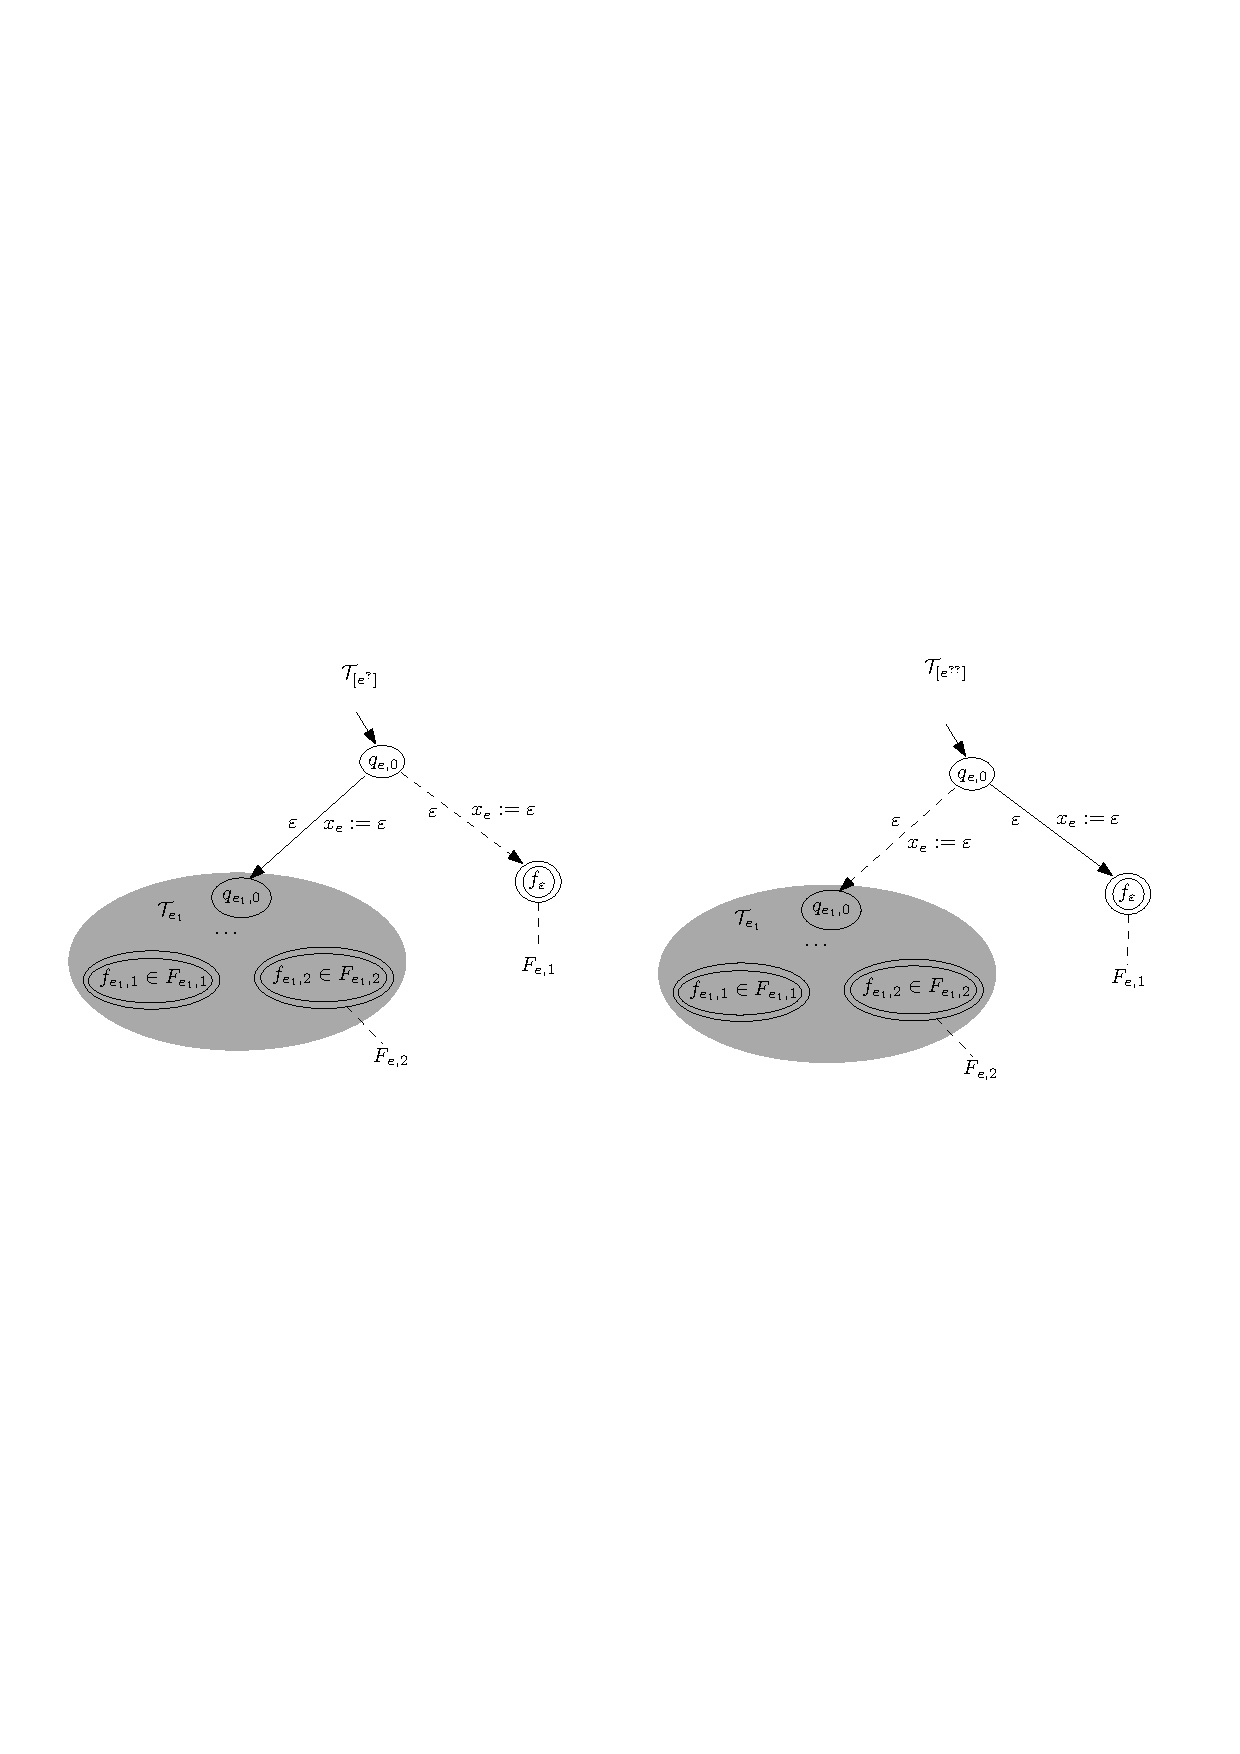
\includegraphics[width = 0.6\textwidth]{reg2pfa-6.pdf}
			\caption{The PFA $\cA_{[e_1^?]}$}
			\label{fig-reg2pfa-6}
		\end{figure}

%%%%%%%%%%%%%%%%%%%%%%%%%%%%%%%%%%%%%%%%%%%%%%%%%%%%%%%%%%%%%%%%%%%%%%%%%%%%%%%%%%%%%%%%%%%%%%%%%%%%%
\paragraph{Case $e = [e_1^{??}]$} 
Let $\cA_{e_1} = (Q_{e_1},
		\Sigma, X, \delta_{e_1}, \tau_{e_1}, E_1 , q_{e_1,0}, (F_{e_1,1}, F_{e_1,2}))$. 
Then 
\[\cA_e = (Q_{e_1} \cup \{q_{e,0}, q_{\varepsilon}\}, \Sigma, X, 
		\delta_e, \tau_e, E, q_{e,0}, (\{q_{\varepsilon}\}, F_{e_1,2}))\] 
where 
		\begin{itemize}
			\item $q_{e,0}  \not \in Q_{e_1}$
			\item $\delta_e(q, a) = \delta_{e_1}(q, a)$ for every $q \in Q_{e_1}$ and $a \in \Sigma$, $\delta_e(q_{e,0}, a)  = ()$ and $\delta_e(q_{\varepsilon}, a) = ()$ for every $a \in \Sigma$, 
			%
			\item $\tau_e(q) = \tau_{e_1}(q)$ for every $q \in Q_{e_1}$, $\tau_e(q_{e,0}) = ((q_{\varepsilon}, q_{e_1,0}); ())$,
			
			\item for each transition $(q, a, q')$ from $\delta_{e_1}$, $E(q,a,q')(x) = E_1(q,a,q')(x)$ and $E(q_{e,0},\varepsilon,q_{\varepsilon})(x) =\varepsilon$
		\end{itemize}
Fig.~\ref{fig-reg2pfa-7} depicts the construction. 
		\begin{figure}[ht]
			\centering
			%\rule{\linewidth}{0cm}
			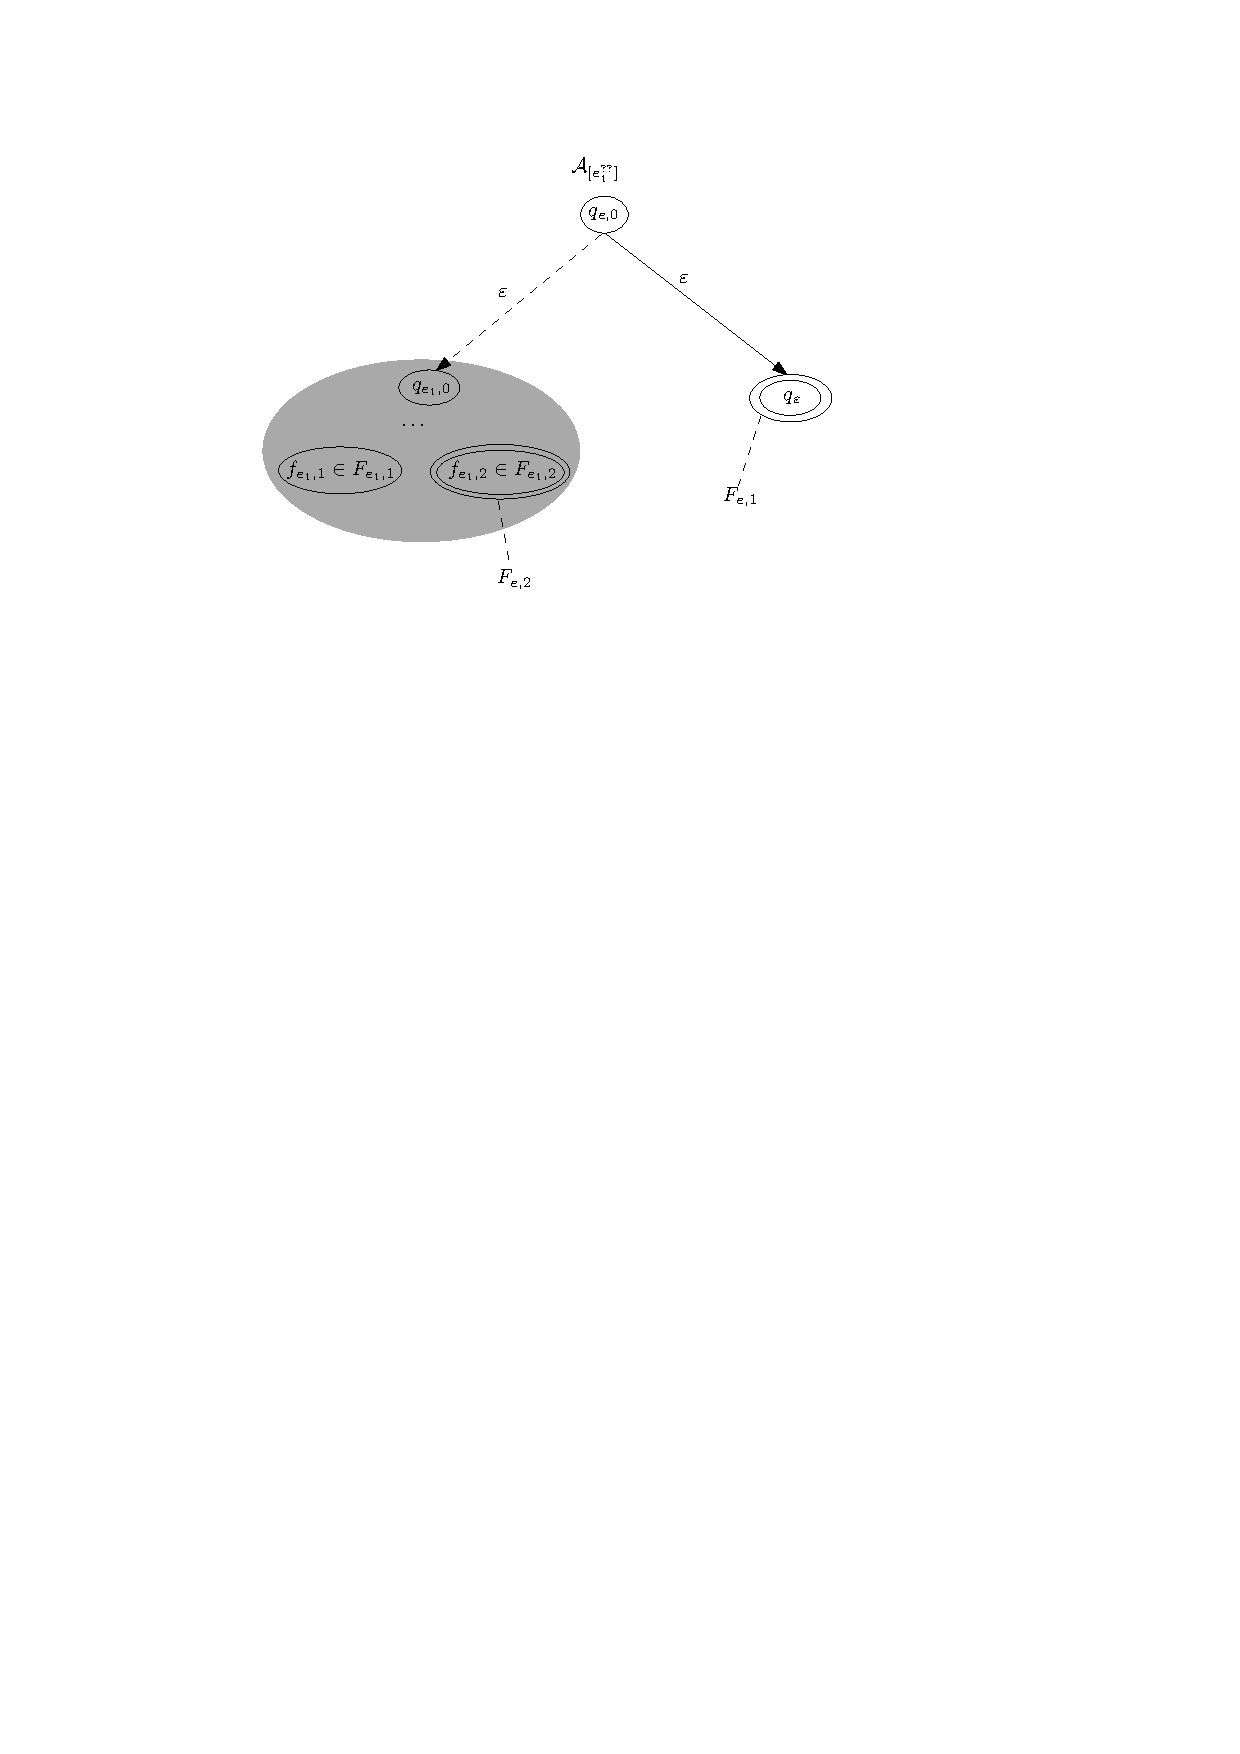
\includegraphics[width = 0.5\textwidth]{reg2pfa-7.pdf}
			\caption{The PFA $\cA_{[e_1^{??}]}$}
			\label{fig-reg2pfa-7}
		\end{figure}
	
%%%%%%%%%%%%%%%%%%%%%%%%%%%%%%%%%%%%%%%%%%%%%%%%%%%%%%%%%%%%%%%%%%%%%%%%%%%%%%%%%%%%%%%%%%%%%%%%%%%%%
\paragraph{Case $e = [e_1 \concat e_2]$} 
Let 
\[\cA_{e_1} = (Q_{e_1}, \Sigma, X_1, \delta_{e_1}, \tau_{e_1}, E_1, q_{e_1,0}, (F_{e_1,1}, F_{e_1,2}))\]
%
\[\cA_{e_2} = (Q_{e_2}, \Sigma, X_2, \delta_{e_2}, \tau_{e_2}, E_2, q_{e_2,0}, (F_{e_2, 1}, F_{e_2,2}))\] and
%
$\cA'_{e_2} = (Q'_{e_2}, \Sigma, X_2, \delta'_{e_2}, \tau'_{e_2}, E_2', q'_{e_2,0}, (F'_{e_2, 1}, F'_{e_2,2}))$ be a fresh copy of $\cA_{e_2}$. Then 
%
\[\cA_e = ( Q_{e_1} \cup Q_{e_2} \cup Q'_{e_2}, \Sigma, X_1\cup X_2 \delta_e, \tau_e, q_{e_1,0}, (F_{e_2,1}, F_{e_2,2} \cup F'_{e_2,1} \cup F'_{e_2,2}))\] where 
	\begin{itemize}
	 \item for every $i \in \{1,2\}$, $q \in Q_{e_i}$ and $a \in \Sigma$, $\delta_e(q, a) = \delta_{e_i}(q, a)$,
			%
	\item for every $q' \in Q'_{e_2}$ and $a \in \Sigma$, $\delta_e(q', a) = \delta'_{e_2}(q',a)$, 
			%    
	\item for every $q \in Q_{e_2}$, $\tau_e(q) = \tau_{e_2}(q)$ and $\tau_e(q') = \tau'_{e_2}(q')$, 
			%
	\item for every $q \in Q_{e_1} \setminus (F_{e_1,1} \cup F_{e_1,2})$, $\tau_e(q) = \tau_{e_1}(q)$, for every $f_{e_1,1} \in F_{e_1,1}$, $\tau_e(f_{e_1,1}) = ((q_{e_2,0}); ())$, and for every $f_{e_1,2} \in F_{e_1,2}$, $\tau_e(f_{e_1,2}) = ((q'_{e_2,0}), ())$,
	%
	\item for $i\in \{1,2\}$, for each transition $(q, a, q')$ from $\delta_{e_i}$  $E(q,a,q')(x) = E_i(q,a,q')(x)$ for $x\in X_i$, and for $x\in X_2$, $E(f_{e_1,1},\varepsilon,q_{e_2,0})(x) =\varepsilon$, $E(f_{e_1,2},\varepsilon,q'_{e_2,0})(x) =\varepsilon$.
  \end{itemize}
 Fig.~\ref{fig-reg2pfa-2} depicts the construction. 
		\begin{figure}[ht]
			\centering
			%\rule{\linewidth}{0cm}
			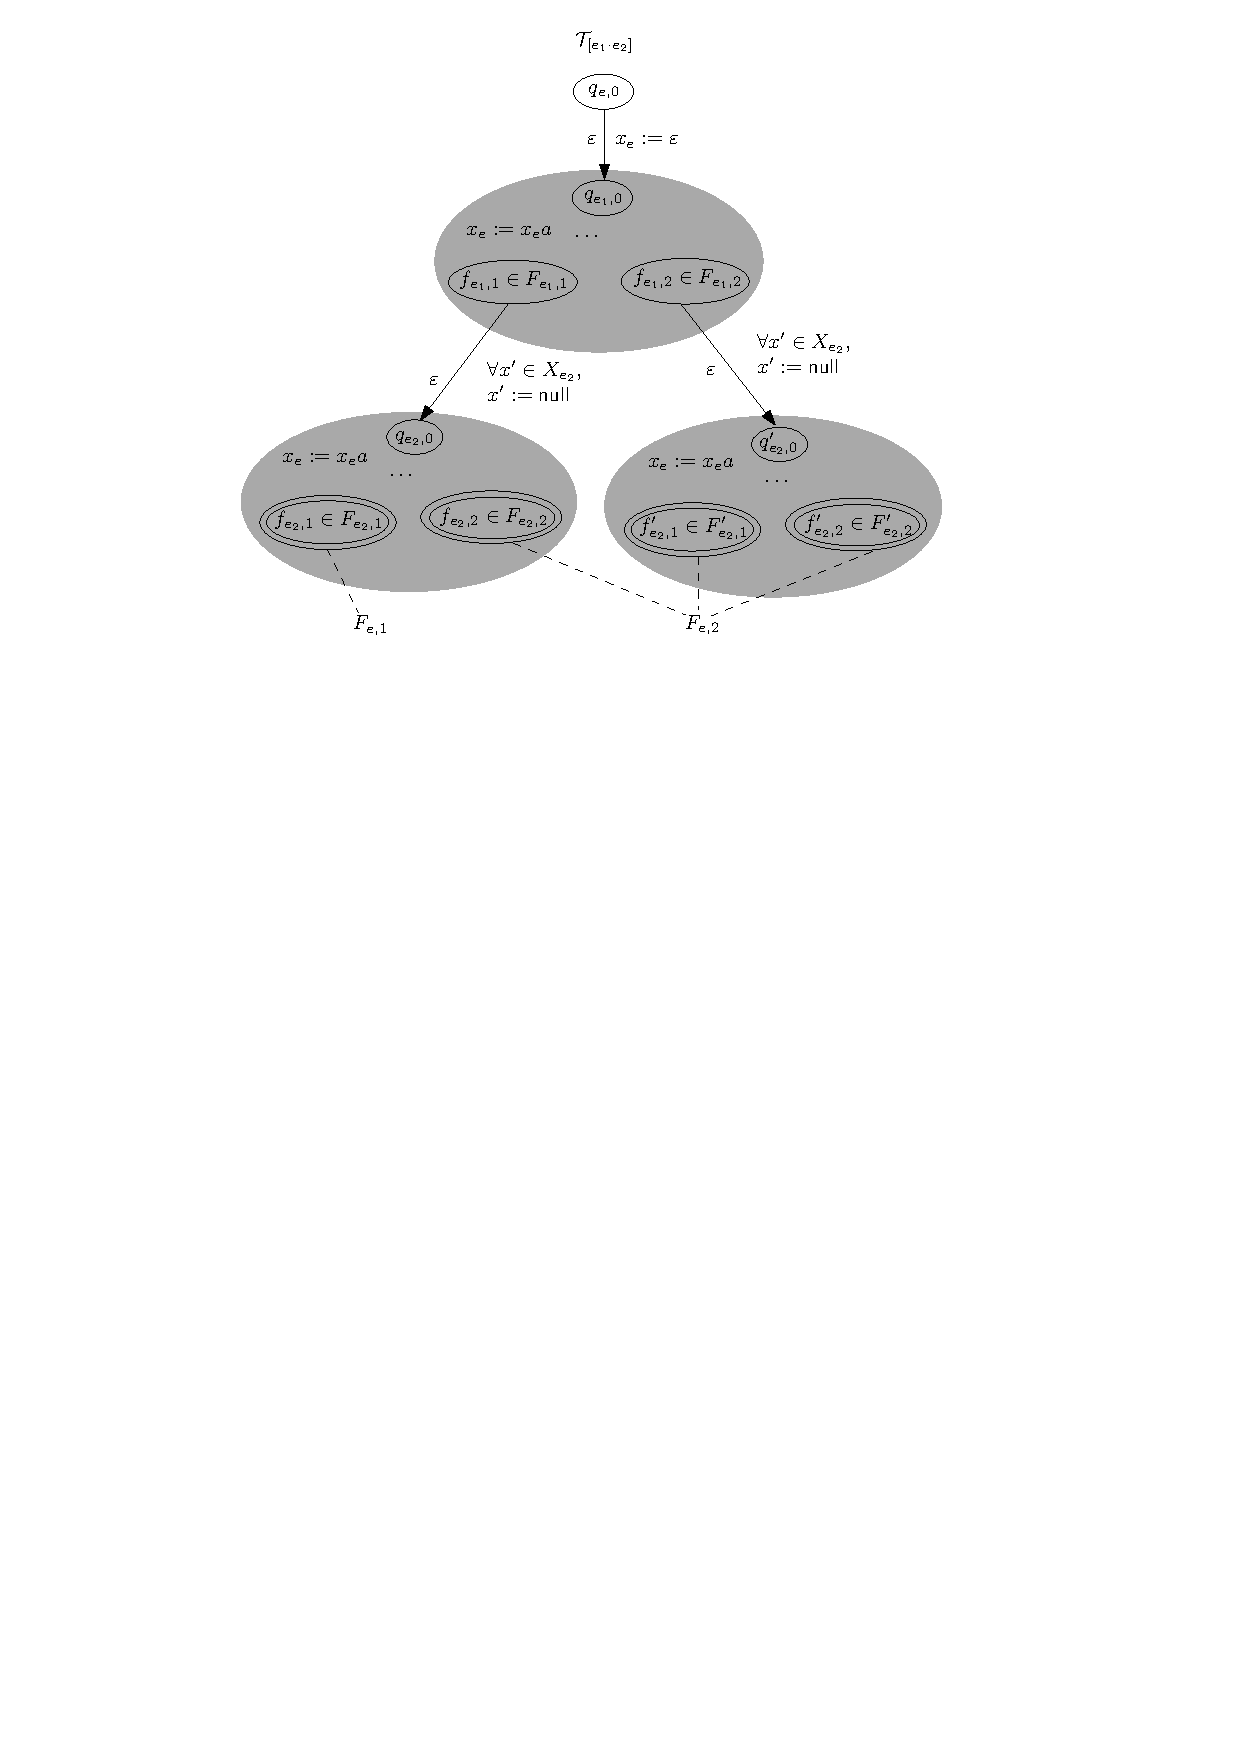
\includegraphics[width = 0.6\textwidth]{reg2pfa-2.pdf}
			\caption{The PFA $\cA_{[e_1\concat e_2]}$}
			\label{fig-reg2pfa-2}
		\end{figure}  
	

%%%%%%%%%%%%%%%%%%%%%%%%%%%%%%%%%%%%%%%%%%%%%%%%%%%%%%%%%%%%%%%%%%%%%%%%%%%%%%%%%%%%%%%%%%%%%%%%%%%%%

\paragraph{Case $e = [e_1^{\ast}]$} 
Let $\cA_{e_1} = (Q_{e_1}, \Sigma, X_1, \delta_{e_1}, \tau_{e_1}, E_1, q_{e_1,0}, (F_{e_1,1}, F_{e_1,2}))$. Then
\[ \cA_e = (Q_{e_1} \cup \{q_{e,0}, f_{e,0}, f_{e,1}\}, \Sigma, X_1, \delta_e, E, \tau_e, q_{e,0}, (\{f_{e,0}\}, \{f_{e,1}\}))\] where 
		\begin{itemize}
			\item $q_{e,0}, f_{e,0} \not \in Q_{e_1}$,
			
			\item for every $q \in Q_{e_1}$ and $a \in \Sigma$, $\delta_e(q, a) = \delta_{e_1}(q, a)$, 
			%moreover, $\delta(q_0, a) = \delta(f_0, a)  = ()$,
			
			\item for every $q \in Q_{e_1} \setminus (F_{e_1,1} \cup F_{e_1,2})$,  $\tau_e(q) = \tau_{e_1}(q)$, moreover, $\tau_e(q_{e,0}) = ((q_{e_1,0},f_{e,0}); ())$,  $\tau_e(q) = ((q_{e_1,0});())$ for every $q \in F_{e_1,1}$, $\tau_e(q) = ((q_{e_1,0}, f_{e,1});())$ for every $q \in F_{e_1,2}$, $\tau_e(f_{e,0}) =\tau_e(f_{e,1}) = (();())$. (Intuitively, the $\varepsilon$-transitions from $q_{e,0}$ to $q_{e_1,0}$ and $f_{e,0}$, from each $q \in F_{e_1,1}$ to $q_{e_1,0}$, and from $q \in F_{e_1,2}$ to $q_{e_1,0}$ and $f_{e,1}$ respectively are added, moreover, the $\varepsilon$-transition from $q_{e,0}$ to $f_{e,0}$ and from $q \in F_{e_1,2}$ to $f_{e,1}$ are of the lowest priority.)
			
			\item for each transition $(q, a, q')$ from $\delta_{e_1}$, $E(q,a,q')(x) = E_1(q,a,q')(x)$, and $E(q_{e,0},\varepsilon,q_{f_e,0})(x) =\varepsilon$, $E(q_{e,0},\varepsilon,q_{e_1,0})(x) =\varepsilon$, $E(f_{e_1,2},\varepsilon,f_{e,1})(x) =x$.
		\end{itemize}

%%%%%%%%%%%%%%%%%%%%%%%%%%%%%%%%%%%%%%%%%%%%%%%%%%%%%%%%%%%%%%%%%%%%%%%%%%%%%%%%%%%%%%%%%%%%%%%%%%%%%
\paragraph{Case $e = [e_1^{+}]$} Then $\cA_e$ is constructed as $\cA_{[e_1 \concat [e^\ast_1]]}$.
		
%%%%%%%%%%%%%%%%%%%%%%%%%%%%%%%%%%%%%%%%%%%%%%%%%%%%%%%%%%%%%%%%%%%%%%%%%%%%%%%%%%%%%%%%%%%%%%%%%%%%%
\paragraph{Case $e = [e_1^{\ast?}]$} Let $\cA_{e_1} = (Q_{e_1}, \Sigma, X_1, \delta_{e_1}, \tau_{e_1}, E_1, q_{e_1,0}, (F_{e_1,1}, F_{e_1,2}))$. 
Then 
\[\cA_e = (Q_{e_1} \cup \{q_{e,0}, f_{e,0}, f_{e,1}\}, \Sigma, X_1, \delta_e, \tau_e, E, q_{e,0}, (\{f_{e,0}\}, \{f_{e,1}\}))\]  
where 
		\begin{itemize}
			\item $q_{e,0}, f_{e,0} \not \in Q_{e_1}$,
			
			\item for every $q \in Q_{e_1}$ and $a \in \Sigma$, $\delta_e(q, a) = \delta_{e_1}(q, a)$, 
			%moreover, $\delta(q_0, a) = \delta(f_0, a)  = ()$,
			
			\item for every $q \in Q_{e_1} \setminus (F_{e_1,1} \cup F_{e_1,2})$,  $\tau_e(q) = \tau_{e_1}(q)$, moreover, $\tau_e(q_{e,0}) = ((f_{e,0}, q_{e_1,0}); ())$,  $\tau_e(q) = ((q_{e_1,0});())$ for every $q \in F_{e_1,1}$, $\tau_e(q) = ((f_{e,1}, q_{e_1,0});())$ for every $q \in F_{e_1,2}$, $\tau_e(f_{e,0}) =\tau_e(f_{e,1}) = (();())$. (Intuitively, the $\varepsilon$-transitions from $q_{e,0}$ to $f_{e,0}$ and $q_{e_1,0}$ , from each $q \in F_{e_1,1}$ to  $q_{e_1,0}$, and from each $q \in F_{e_1,2}$ to $f_{e,1}$ and $q_{e_1,0}$ respectively are added, moreover, the $\varepsilon$-transition from $q_{e,0}$ to $q_{e_1,0}$ and from $q \in F_{e_1,2}$ to $q_{e_1,0}$ are of the lowest priority.)
			
			\item for each transition $(q, a, q')$ from $\delta_{e_1}$, $E(q,a,q')(x) = E_1(q,a,q')(x)$, and $E(q_{e,0},\varepsilon,q_{f_e,0})(x) =\varepsilon$, $E(q_{e,0},\varepsilon,q_{e_1,0})(x) =\varepsilon$, $E(f_{e_1,2},\varepsilon,f_{e,1})(x) =x$.
		\end{itemize}

 
%%%%%%%%%%%%%%%%%%%%%%%%%%%%%%%%%%%%%%%%%%%%%%%%%%%%%%%%%%%%%%%%%%%%%%%%%%%%%%%%%%%%%%%%%%%%%%%%%%%%%
\paragraph{Case $e = [e_1^{+?}]$} then $\cA_e$ is constructed as $\cA_{[e_1 \concat [e_1^{*?}]]}$.

Fig.~\ref{fig-reg2pfa-3} depicts the construction. 
\begin{figure}[ht]
	\centering
	%\rule{\linewidth}{0cm}
	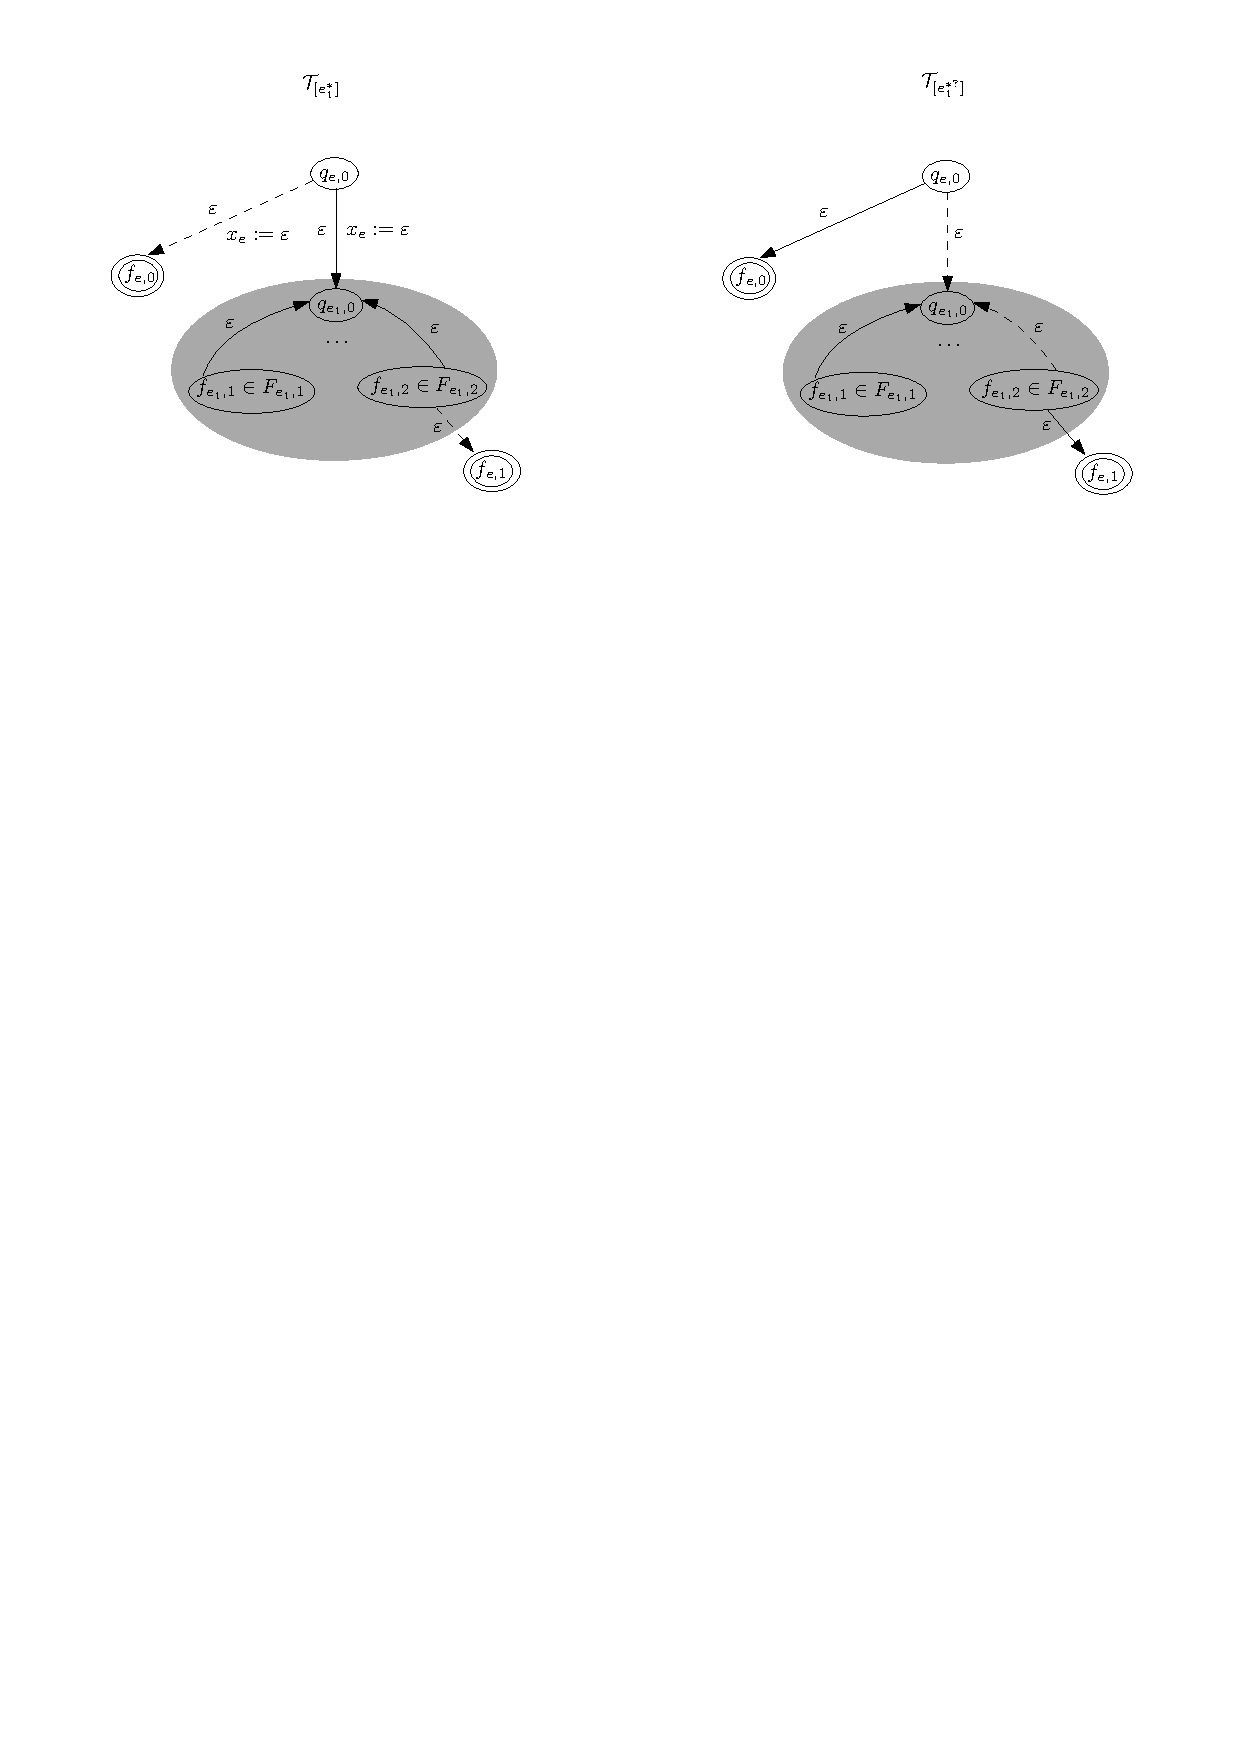
\includegraphics[width = 0.8\textwidth]{reg2pfa-3.pdf}
	\caption{The PFA $\cA_{[e_1^\ast]}$ and $\cA_{[e_1^{\ast?}]}$}
	\label{fig-reg2pfa-3}
\end{figure}

%%%%%%%%%%%%%%%%%%%%%%%%%%%%%%%%%%%%%%%%%%%%%%%%%%%%%%%%%%%%%%%%%%%%%%%%%%%%%%%%%%%%%%%%%%%%%%%%%%%%%
\paragraph{Case $e = [e_1^{\{m_1,m_2\}}]$} Then $\cA_e$ is constructed as the concatenation of $\cA_{e_1^{m_1}}$ and $\cA^\prime_{e_1^{\{1,m_2-m_1\}}}$, where $\cA_{e_1^{m_1}}$ is the PFA corresponding to consecutive concatenations of $m_1$ copies of $e_1$, and $\cA^\prime_{e_1^{\{1,m_2-m_1\}}}$ is illustrated in Fig.~\ref{fig-reg2pfa-4}, which consists of $m_2-m_1$ copies of $\cA_{e_1}$, say $(\cA^{(i)}_{e_1})_{i \in [m_2-m_1]}$, as well as the $\varepsilon$-transition from $q^{(1)}_{e_1,0}$ to a fresh state $f^\prime_0$ (of the lowest priority), and the $\varepsilon$-transitions from each $f^{(i)}_{e_1,2} \in F^{(i)}_{e_1,2}$ to $q^{(i+1)}_{e_1,0}$ (of the highest priority), and a fresh state $f^\prime_1$ (of the lowest priority). The accepting states of $\cA^\prime_{e_1^{\{1,m_2-m_1\}}}$ are $(\{f_0'\},\{f_1'\})$. (Intuitively, each $\cA^{(i)}_{e_1}$ accepts only nonempty strings, thus $f^{(i)}_{e_1,1} \in F^{(i)}_{e_1,1}$ contains no outgoing transitions in $\cA^\prime_{e_1^{\{1,m_2-m_1\}}}$. )
		%
		\begin{figure}[ht]
			\centering
			%\rule{\linewidth}{0cm}
			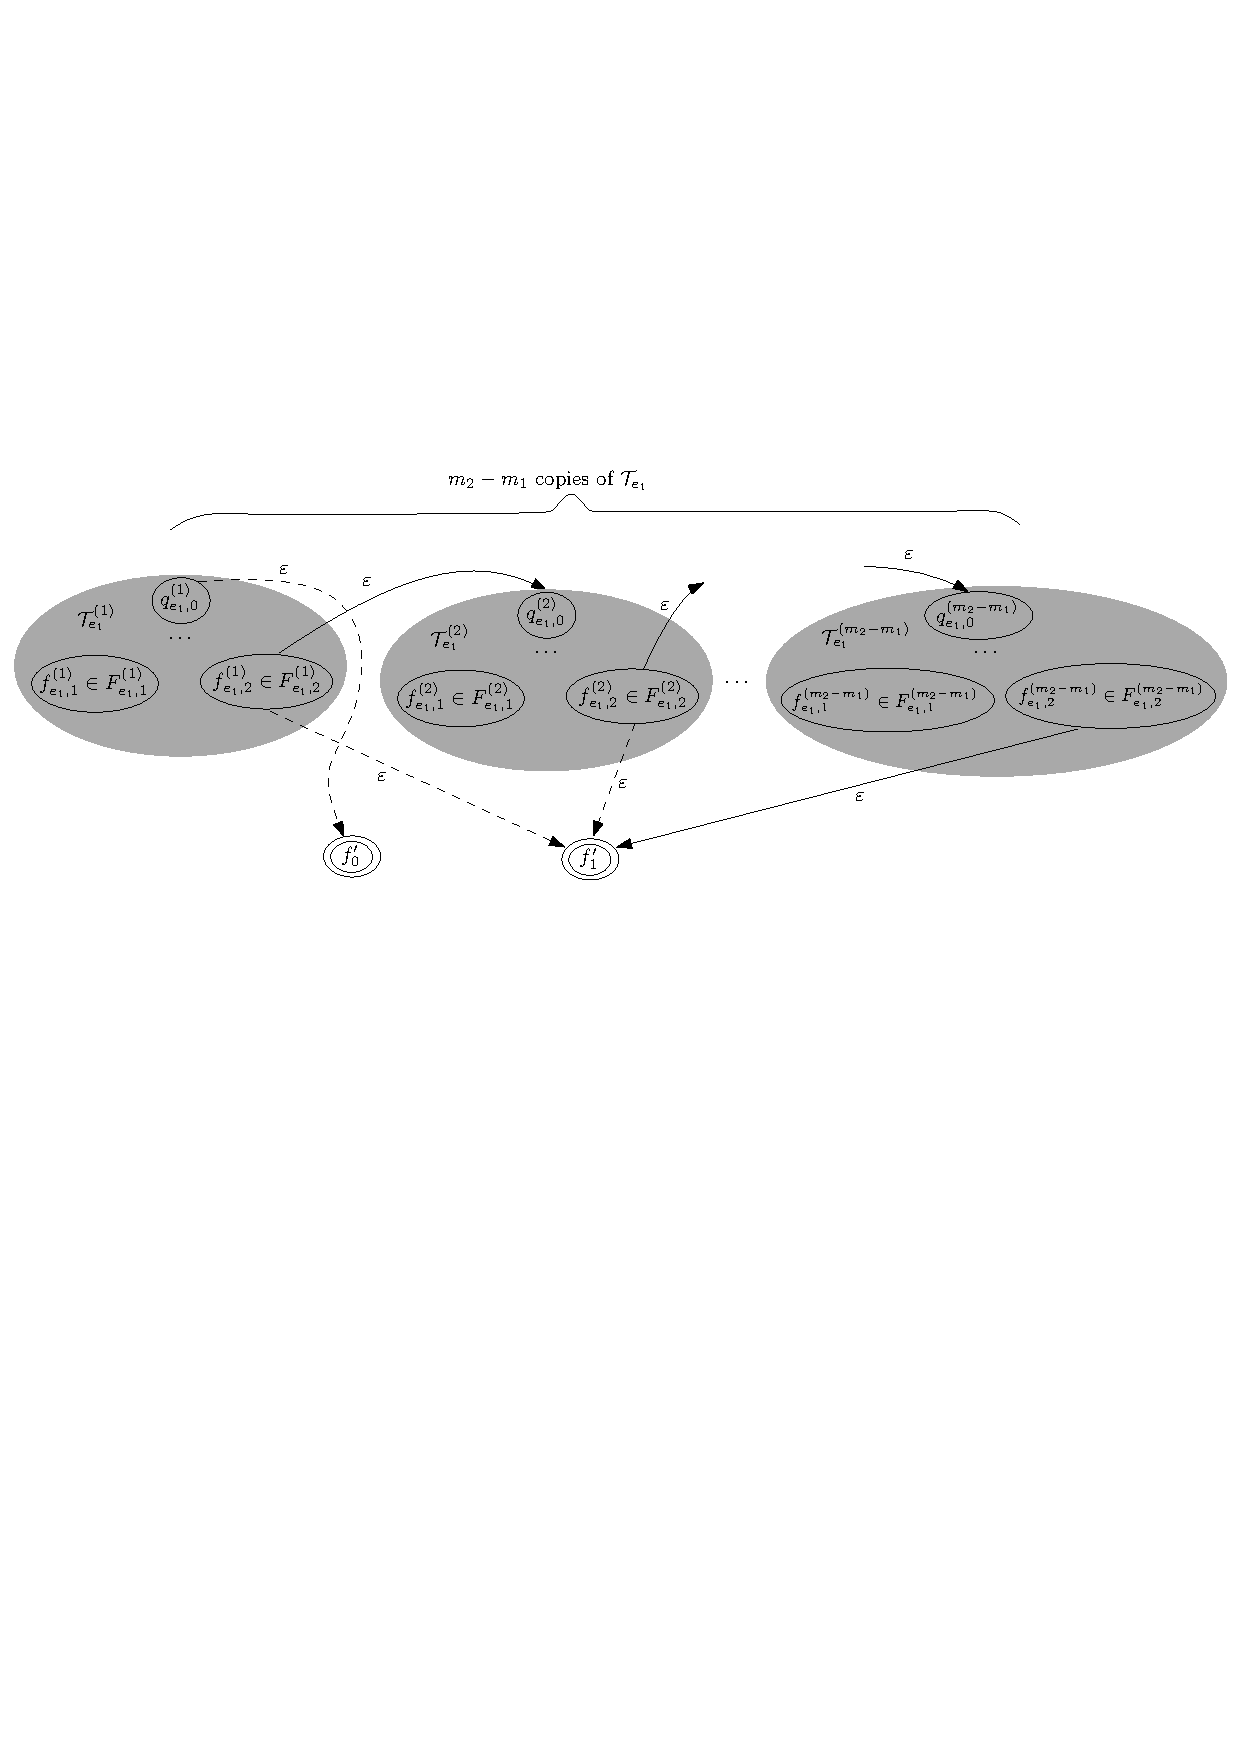
\includegraphics[width = 0.8\textwidth]{reg2pfa-4.pdf}
			\caption{The PFA $\cA^\prime_{e_1^{\{1,m_2-m_1\}}}$}
			\label{fig-reg2pfa-4}
		\end{figure}  


%%%%%%%%%%%%%%%%%%%%%%%%%%%%%%%%%%%%%%%%%%%%%%%%%%%%%%%%%%%%%%%%%%%%%%%%%%%%%%%%%%%%%%%%%%%%%%%%%%%%%
\paragraph{Case $e = [e_1^{\{m_1,m_2\}?}]$} Then $\cA_e$ is constructed as the concatenation of $\cA_{e_1^{m_1}}$ and $\cA^\prime_{e_1^{\{1,m_2-m_1\}?}}$, where $\cA^\prime_{e_1^{\{1,m_2-m_1\}?}}$ is illustrated in Fig.~\ref{fig-reg2pfa-5}, which is the same as $\cA^\prime_{e_1^{\{1,m_2-m_1\}}}$ in Fig.~\ref{fig-reg2pfa-4}, except that the priorities of $\varepsilon$-transition from $q^{(1)}_{e_1,0}$ to $f^\prime_0$ has the highest priority and  the priorities of $\varepsilon$-transitions from each $f^{(i)}_{e_1,2} \in F^{(i)}_{e_1,2}$ to $f^\prime_1$ are reversed.
		\begin{figure}[ht]
			\centering
			%\rule{\linewidth}{0cm}
			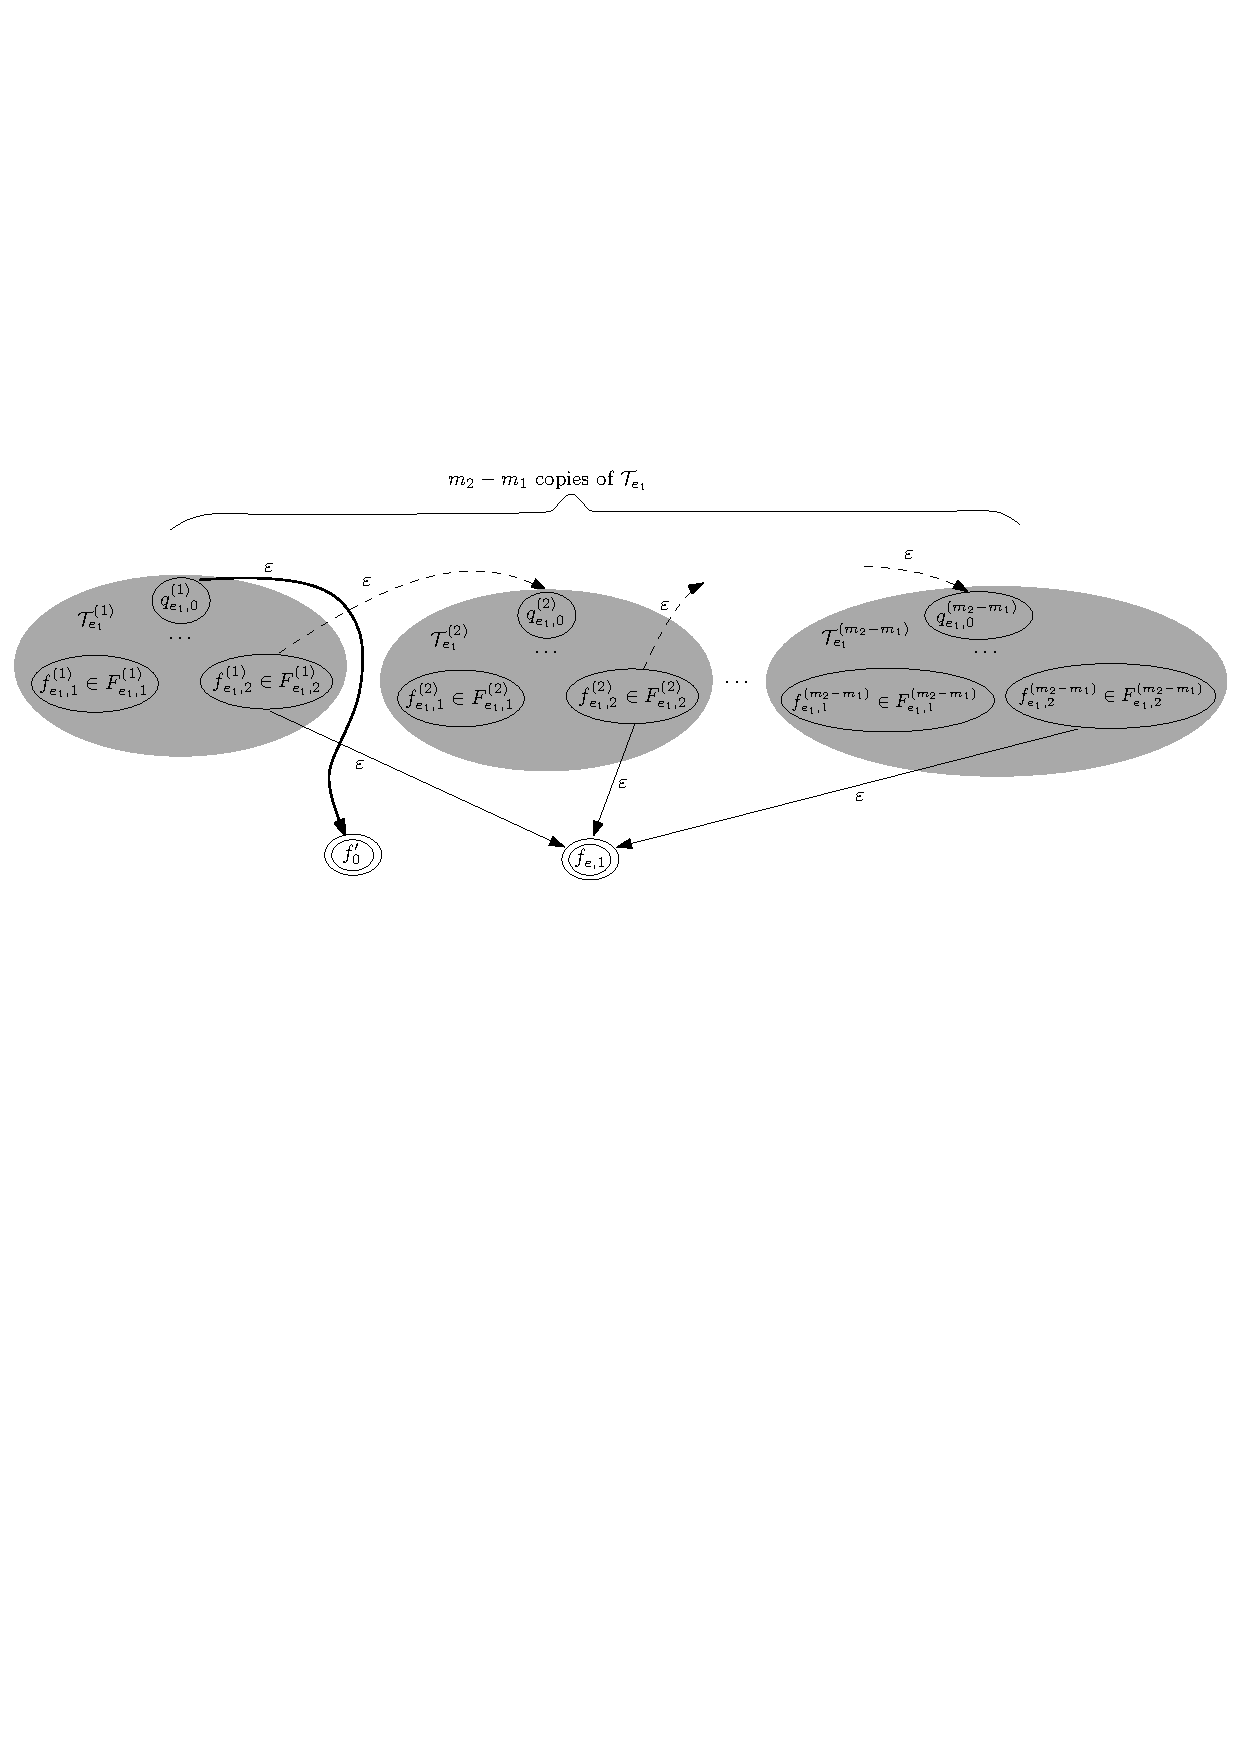
\includegraphics[width = 0.8\textwidth]{reg2pfa-5.pdf}
			\caption{The PFA $\cA^\prime_{e_1^{\{1,m_2-m_1\}?}}$}
			\label{fig-reg2pfa-5}
		\end{figure}  
%%%%%%%%%%%%%%%%%%%%%%%%%%%%%%%%%%%%%%%%%%%%%%%%%%%%%%%%%%%%%%%%%%%%%%%%%%%%%%%%%%%%%%%%%%%%%%%%%%%%%%%%

 %can be constructed 
%(in linear time)

% such that 
%	\begin{itemize}
%		\item $\cA_e$ has a unique initial state without incoming transitions and a unique final state without outgoing transitions,
%		%
%		\item for subexpression $e'$ of $e$, $\cA_e$ contains at least one isomorphic copy of $\cA_{e'}$ (i.e. the PFA constructed for $e'$), denoted by ${\sf Sub}_{e'}[\cA_e]$. 
%	\end{itemize}

%Let us use ${\sf Sub}_{e'}[\cA_e]$ to denote the isomorphic copy of $\cA_{e'}$ in $\cA_e$, as mentioned in Proposition~\ref{prop-rwre-to-pfa}.

%\begin{proof}
%	For any $e \in \cgexp$, a PFA $\cA_e$ is constructed recursively in the sequel. The constructed PFA $\cA_e$ satisfies that 
%	\begin{itemize}
%		\item it has a unique initial state without incoming transitions and each of its final states has no outgoing transitions,
%		\item all the transitions out of the initial state are $\varepsilon$-transitions, 
%		\item the set of final states is divided into two disjoint subsets $F_1, F_2$ such that for each $w \in \Sigma^*$ satisfying that $q_0 \xrightarrow[\cA_e]{w} q$ for some $q \in F_1$ (resp. $q \in F_2$), $w = \varepsilon$ (resp. $w \neq \varepsilon$).
%	\end{itemize}



\begin{example}\label{exmp-pfa}
	The PFA corresponding to the RWRE $e = [[([\Gamma^+])\concat .?] \concat ([\Gamma^*])]$ 
	%in Example~\ref{exmp-regex-match-tree}
	%
	is illustrated in Fig.~\ref{fig-pfa}, where the dashed (resp. thicker solid) lines represent the $\varepsilon$-transitions of lower (resp. higher) priorities than non-$\varepsilon$ transitions (if there is any), and the doubly circled states are final states. For instance, $\delta(q_1, \ell) = (q_1)$ for every $\ell \in \{0, \dots, 9\}$, $\delta(q_1, .) = ()$, $\tau(q_1) = ((); (q_2))$. Since the $\varepsilon$-transition has lower priority than the $\ell$-transition at the state $q_1$, whenever the currently scanned letter is $\ell \in \{0,\cdots,9\}$ at $q_1$,  the PFA will choose to go to $q_1$ greedily, until there is no more $\ell  \in \{0,\cdots,9\}$. (In this case, it has to choose the $\epsilon$-transition and goes to $q_2$.)
	%
	\begin{figure}[ht]
		
		\centering
		%\rule{\linewidth}{0cm}
		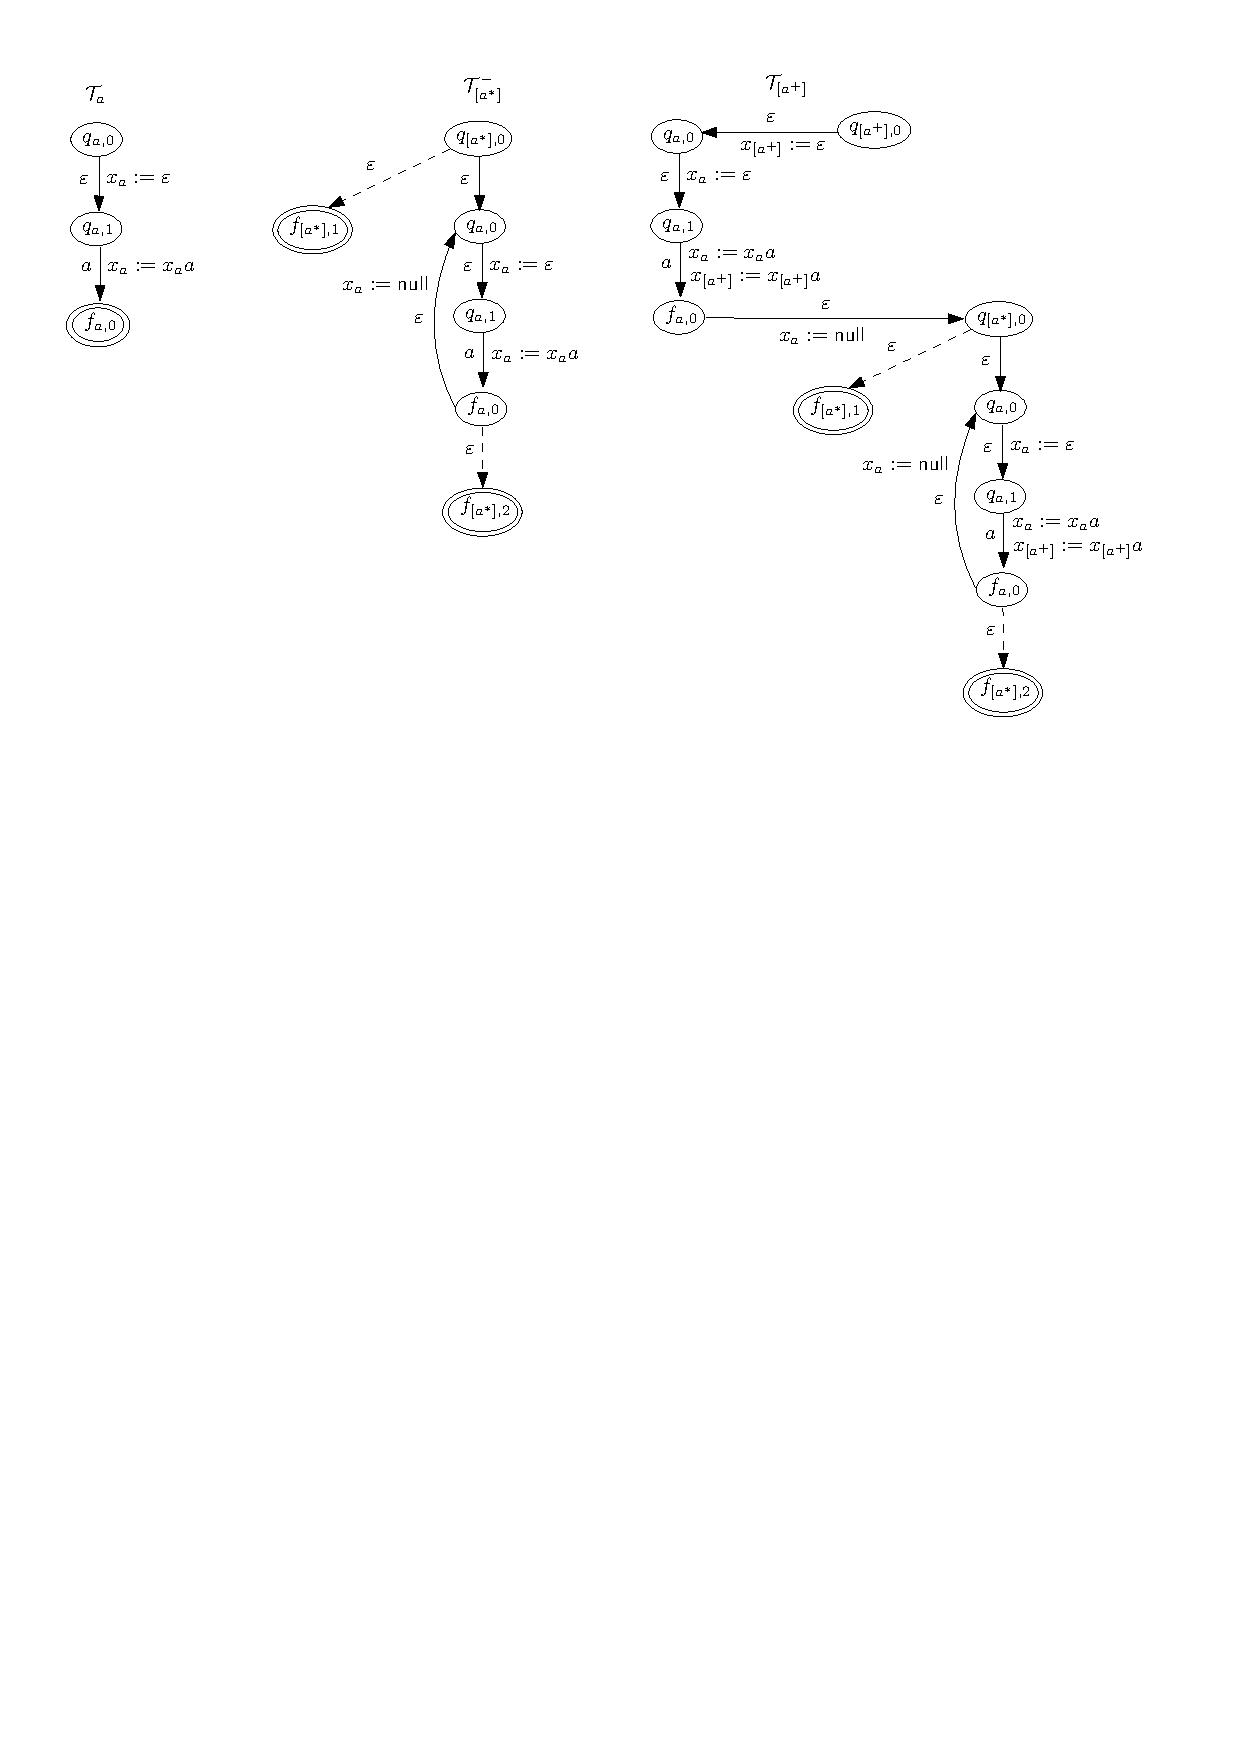
\includegraphics[width=0.9\textwidth]{pfa-new.pdf}
		\caption{The PFA for $e = [[([\Gamma^+])\concat .?] \concat ([\Gamma^*])]$, where $\Gamma = \{0, \cdots, 9\}$}
		\label{fig-pfa}
		
	\end{figure}
\end{example}

